\section{Anexos}\label{anexos}

\subsection{Formato de Encuesta}\label{formato-de-encuesta}

\begin{figure}[H]
    \begin{flushleft}
        \textbf{Figura Anexo C1}\\
        \emph{Formato Cuestionario en Blanco 1}
    \end{flushleft}
    \vspace{0.1cm}
    \centering
    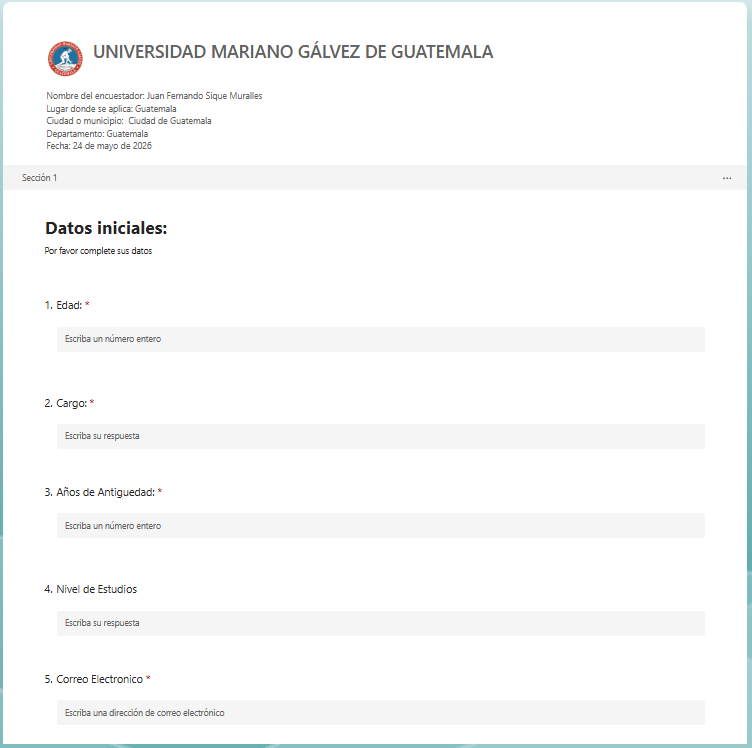
\includegraphics[width=\textwidth]{./imagenes/image8.png}
\end{figure}

\begin{figure}[H]
    \begin{flushleft}
        \textbf{Figura Anexo C2}\\
        \emph{Formato cuestionario en Blanco 2}
    \end{flushleft}
    \vspace{0.1cm}
    \centering
    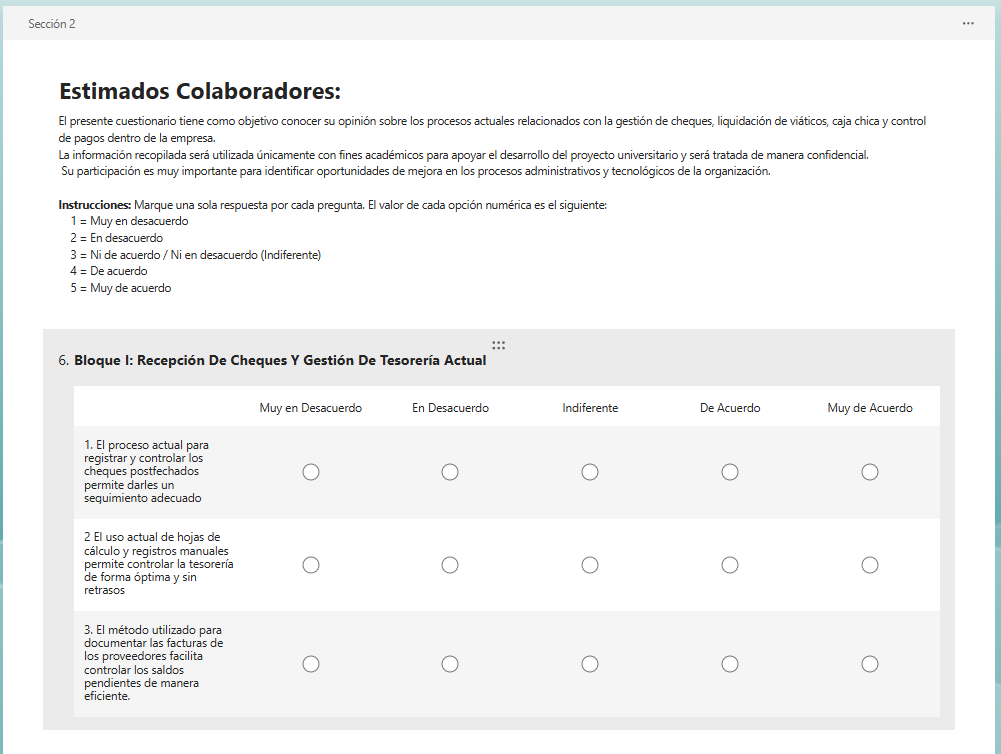
\includegraphics[width=\textwidth]{./imagenes/image9.png}
\end{figure}

\begin{figure}[H]
    \begin{flushleft}
        \textbf{Figura Anexo C3}\\
        \emph{Formato cuestionario en Blanco 3}
    \end{flushleft}
    \vspace{0.1cm}
    \centering
    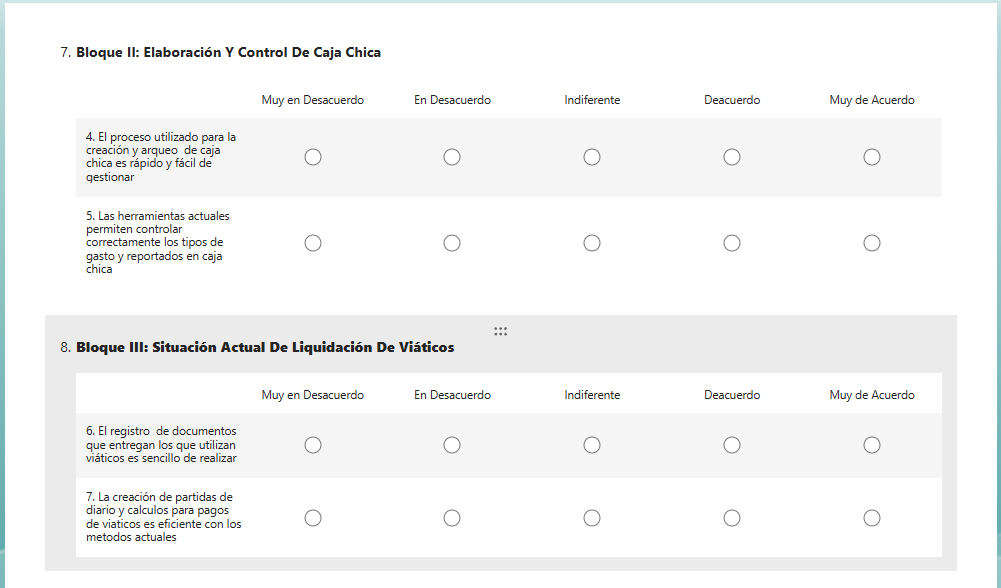
\includegraphics[width=\textwidth]{./imagenes/image10.png}
\end{figure}

\begin{figure}[H]
    \begin{flushleft}
        \textbf{Figura Anexo C4}\\
        \emph{Formato cuestionario en Blanco 4}
    \end{flushleft}
    \vspace{0.1cm}
    \centering
    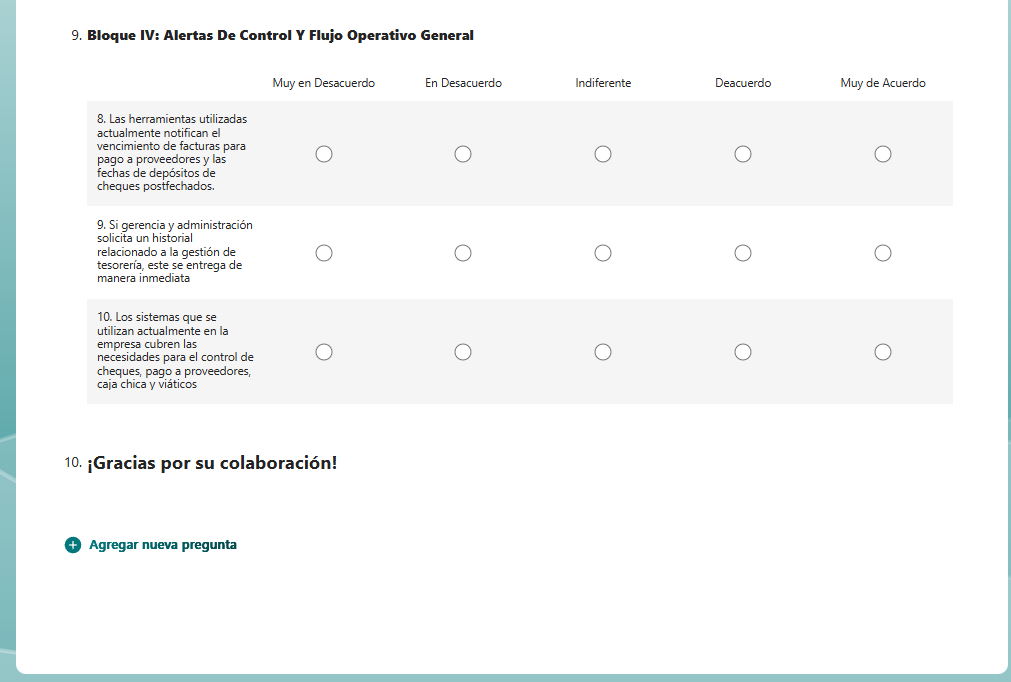
\includegraphics[width=\textwidth]{./imagenes/image11.png}
\end{figure}

\subsection{Muestra de Aplicación}\label{muestra-de-aplicacion}

\begin{figure}[H]
    \begin{flushleft}
        \textbf{Figura Anexo C5}\\
        \emph{Formato cuestionario 1 lleno 1}
    \end{flushleft}
    \vspace{0.1cm}
    \centering
    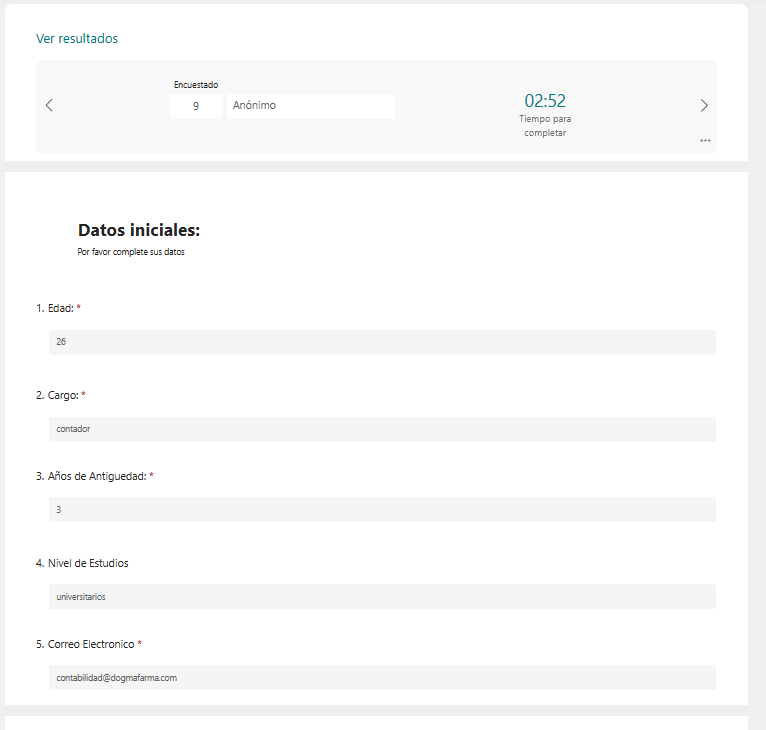
\includegraphics[width=\textwidth]{./imagenes/image12.png}
\end{figure}

\begin{figure}[H]
    \begin{flushleft}
        \textbf{Figura Anexo C6}\\
        \emph{Formato cuestionario 1 lleno 2}
    \end{flushleft}
    \vspace{0.1cm}
    \centering
    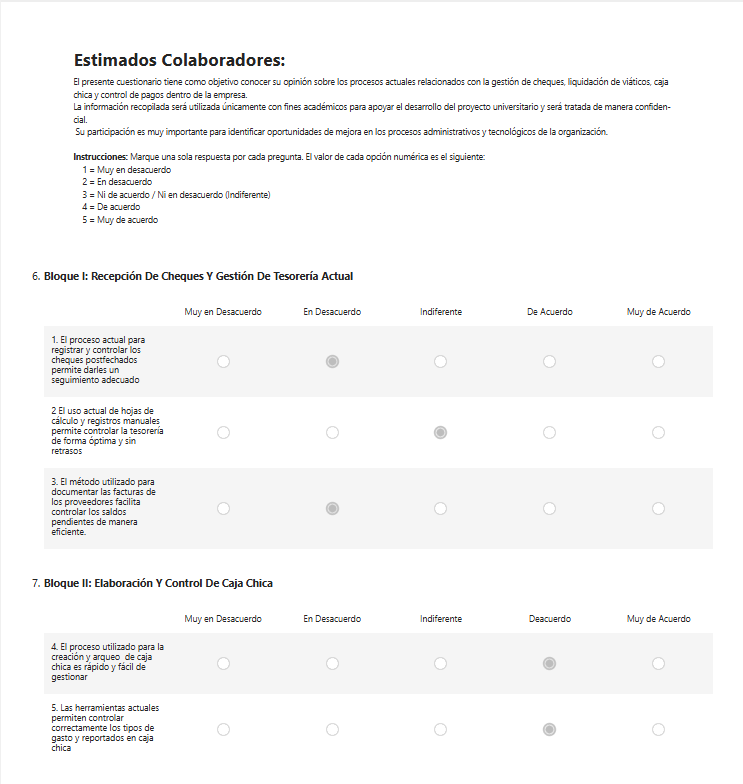
\includegraphics[width=\textwidth]{./imagenes/image13.png}
\end{figure}

\begin{figure}[H]
    \begin{flushleft}
        \textbf{Figura Anexo C7}\\
        \emph{Formato cuestionario 1 lleno 3}
    \end{flushleft}
    \vspace{0.1cm}
    \centering
    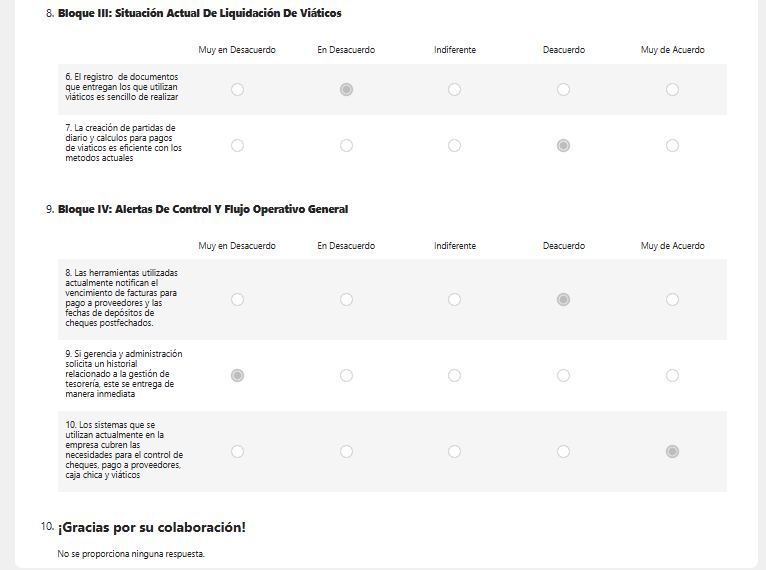
\includegraphics[width=\textwidth]{./imagenes/image14.png}
\end{figure}

\begin{figure}[H]
    \begin{flushleft}
        \textbf{Figura Anexo C8}\\
        \emph{Formato cuestionario 2 lleno 1}
    \end{flushleft}
    \vspace{0.1cm}
    \centering
    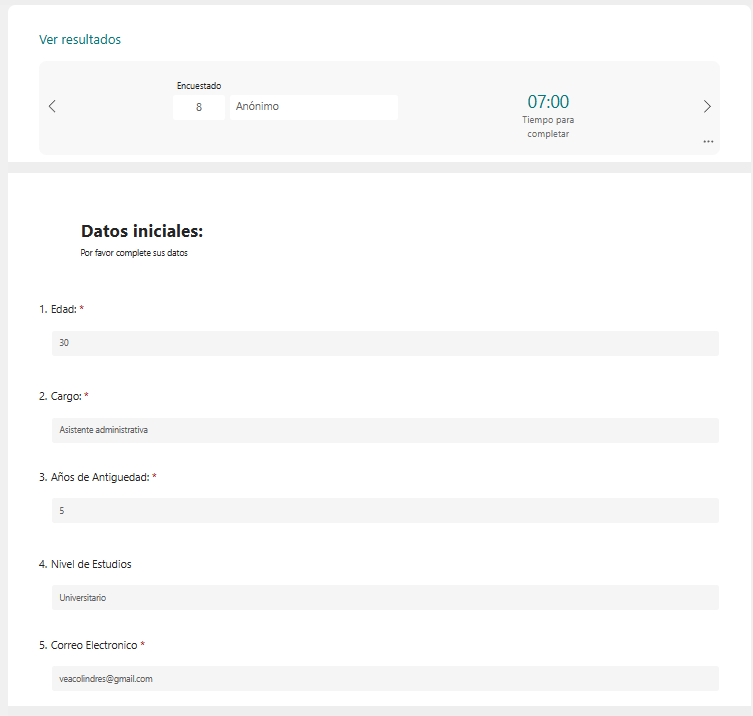
\includegraphics[width=\textwidth]{./imagenes/image15.png}
\end{figure}

\begin{figure}[H]
    \begin{flushleft}
        \textbf{Figura Anexo C9}\\
        \emph{Formato cuestionario 2 lleno 2}
    \end{flushleft}
    \vspace{0.1cm}
    \centering
    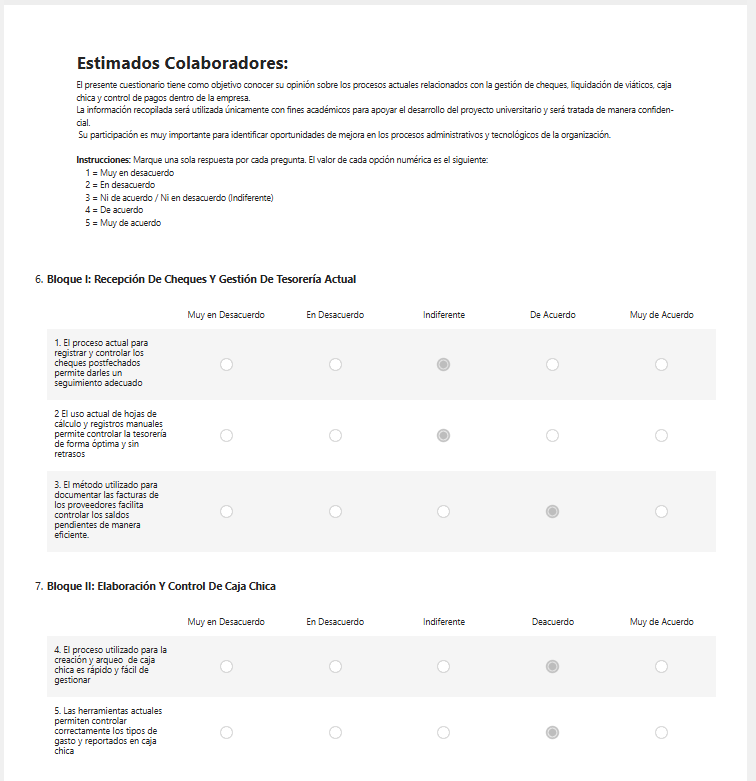
\includegraphics[width=\textwidth]{./imagenes/image16.png}
\end{figure}

\begin{figure}[H]
    \begin{flushleft}
        \textbf{Figura Anexo C10}\\
        \emph{Formato cuestionario 2 lleno 3}
    \end{flushleft}
    \vspace{0.1cm}
    \centering
    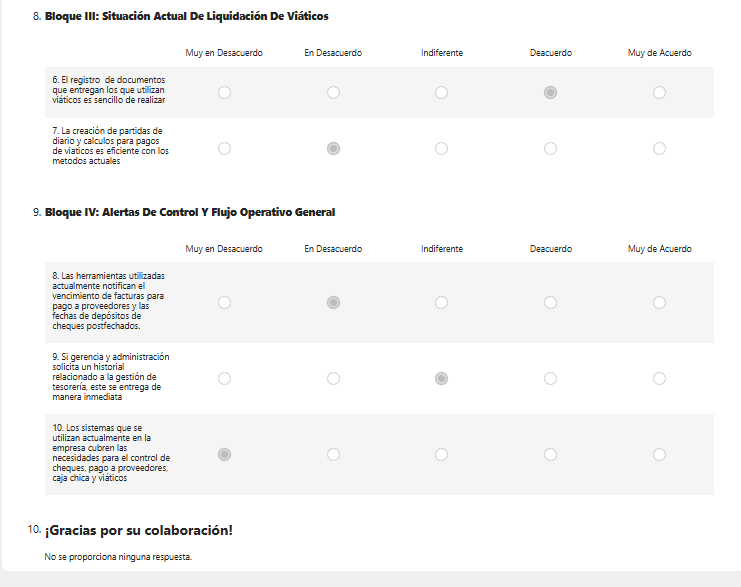
\includegraphics[width=\textwidth]{./imagenes/image17.png}
\end{figure}

\subsection{Interpretación de Escala de Likert}\label{interpretacion-de-escala-de-likert}

\begin{figure}[H]
    \begin{flushleft}
        \textbf{Figura Anexo C11}\\
        \emph{Resultado de la Escala de Likert}
    \end{flushleft}
    \vspace{0.1cm}
    \centering
    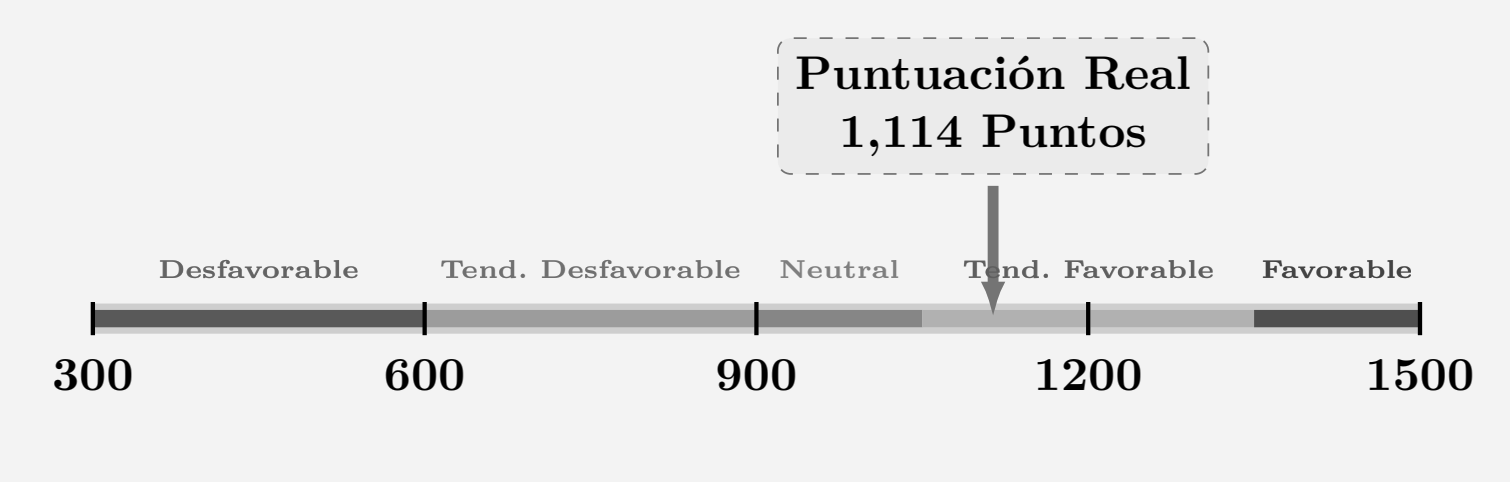
\includegraphics[width=\textwidth]{./imagenes/image18.png}
\end{figure}

\begin{figure}[H]
    \begin{flushleft}
        \textbf{Figura Anexo C12}\\
        \emph{Bloque I}
    \end{flushleft}
    \vspace{0.1cm}
    \centering
    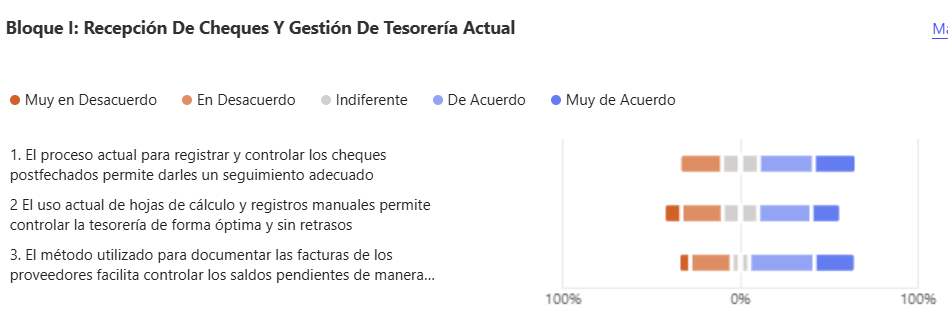
\includegraphics[width=\textwidth]{./imagenes/image19.png}
\end{figure}

\begin{table}[H]
\small
\begin{flushleft}
    \textbf{Tabla Anexo C1}\\[0.2cm]
    \emph{Bloque I (Porcentajes Tres preguntas)}
\end{flushleft}
\renewcommand{\arraystretch}{1.0}
\centering
\begin{tabular}{
    >{\raggedright\arraybackslash}p{2.6cm} 
    >{\raggedright\arraybackslash}p{1.6cm} 
    >{\raggedright\arraybackslash}p{1.6cm} 
    >{\raggedright\arraybackslash}p{1.6cm} 
    >{\raggedright\arraybackslash}p{2.0cm} 
    >{\raggedright\arraybackslash}p{2.3cm} 
    >{\raggedright\arraybackslash}p{1.8cm}
}
\toprule
\textbf{Preguntas} & \textbf{Muy de\newline Acuerdo} & \textbf{De\newline Acuerdo} & \textbf{Indiferente} & \textbf{En\newline Desacuerdo} & \textbf{Muy en\newline Desacuerdo} & \textbf{Sin\newline Respuesta} \\
\midrule
P.1 & 7 & 9 & 6 & 7 & 0 & 1 \\
P.2 & 5 & 9 & 6 & 7 & 3 & 0 \\
P.3 & 7 & 11 & 3 & 7 & 2 & 0 \\
\midrule
\textbf{Suma Bloque} & \textbf{19} & \textbf{29} & \textbf{15} & \textbf{21} & \textbf{5} & \textbf{1} \\
\textbf{Total (\%)} & \textbf{21.1\%} & \textbf{32.2\%} & \textbf{16.7\%} & \textbf{23.3\%} & \textbf{5.6\%} & \textbf{1.1\%} \\
\bottomrule
\end{tabular}
\end{table}

\begin{figure}[H]
    \begin{flushleft}
        \textbf{Figura Anexo C13}\\
        \emph{Bloque II}
    \end{flushleft}
    \vspace{0.1cm}
    \centering
    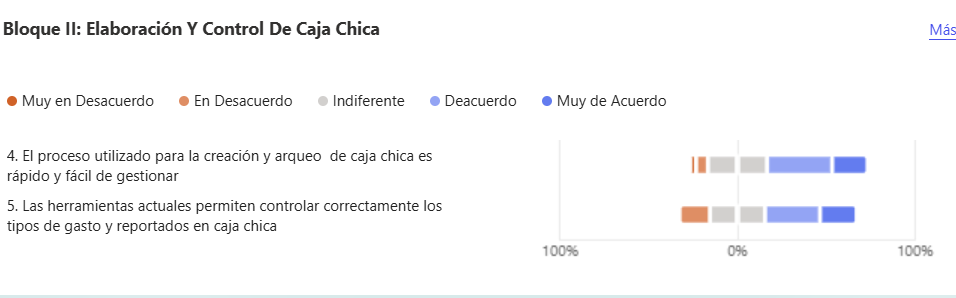
\includegraphics[width=\textwidth]{./imagenes/image20.png}
\end{figure}

\begin{table}[H]
\small
\begin{flushleft}
    \textbf{Tabla Anexo C2}\\[0.2cm]
    \emph{Bloque II (Porcentajes dos preguntas)}
\end{flushleft}
\renewcommand{\arraystretch}{1.0}
\centering
\begin{tabular}{
    >{\raggedright\arraybackslash}p{2.6cm} 
    >{\raggedright\arraybackslash}p{1.6cm} 
    >{\raggedright\arraybackslash}p{1.6cm} 
    >{\raggedright\arraybackslash}p{1.6cm} 
    >{\raggedright\arraybackslash}p{2.0cm} 
    >{\raggedright\arraybackslash}p{2.3cm} 
    >{\raggedright\arraybackslash}p{1.8cm}
}
\toprule
\textbf{Preguntas} & \textbf{Muy de\newline Acuerdo} & \textbf{De\newline Acuerdo} & \textbf{Indiferente} & \textbf{En\newline Desacuerdo} & \textbf{Muy en\newline Desacuerdo} & \textbf{Sin\newline Respuesta} \\
\midrule
P.4 & 6 & 11 & 10 & 2 & 1 & 0 \\
P.5 & 6 & 9 & 9 & 5 & 0 & 1 \\
\midrule
\textbf{Suma Bloque} & \textbf{12} & \textbf{20} & \textbf{19} & \textbf{7} & \textbf{1} & \textbf{1} \\
\textbf{Total (\%)} & \textbf{20.0\%} & \textbf{33.3\%} & \textbf{31.7\%} & \textbf{11.7\%} & \textbf{1.7\%} & \textbf{1.6\%} \\
\bottomrule
\end{tabular}
\end{table}

\begin{figure}[H]
    \begin{flushleft}
        \textbf{Figura Anexo C14}\\
        \emph{Bloque III}
    \end{flushleft}
    \vspace{0.1cm}
    \centering
    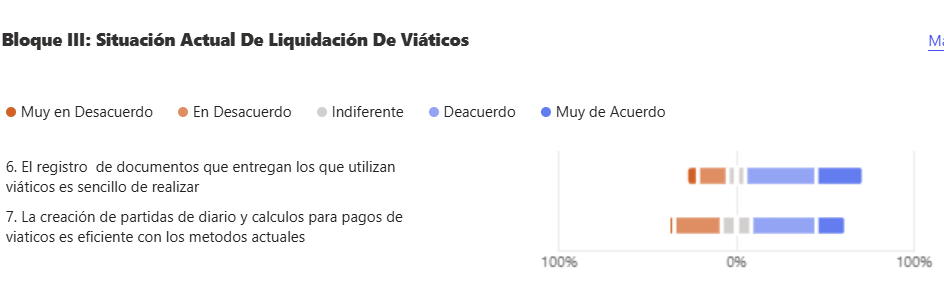
\includegraphics[width=\textwidth]{./imagenes/image21.png}
\end{figure}

\begin{table}[H]
\small
\begin{flushleft}
    \textbf{Tabla Anexo C3}\\[0.2cm]
    \emph{Bloque III (Porcentajes Dos preguntas)}
\end{flushleft}
\renewcommand{\arraystretch}{1.0}
\centering
\begin{tabular}{
    >{\raggedright\arraybackslash}p{2.6cm} 
    >{\raggedright\arraybackslash}p{1.6cm} 
    >{\raggedright\arraybackslash}p{1.6cm} 
    >{\raggedright\arraybackslash}p{1.6cm} 
    >{\raggedright\arraybackslash}p{2.0cm} 
    >{\raggedright\arraybackslash}p{2.3cm} 
    >{\raggedright\arraybackslash}p{1.8cm}
}
\toprule
\textbf{Preguntas} & \textbf{Muy de\newline Acuerdo} & \textbf{De\newline Acuerdo} & \textbf{Indiferente} & \textbf{En\newline Desacuerdo} & \textbf{Muy en\newline Desacuerdo} & \textbf{Sin\newline Respuesta} \\
\midrule
P.6 & 8 & 12 & 3 & 5 & 2 & 0 \\
P.7 & 5 & 11 & 5 & 8 & 1 & 0 \\
\midrule
\textbf{Suma Bloque} & \textbf{13} & \textbf{23} & \textbf{8} & \textbf{13} & \textbf{3} & \textbf{0} \\
\textbf{Total (\%)} & \textbf{21.7\%} & \textbf{38.3\%} & \textbf{13.3\%} & \textbf{21.7\%} & \textbf{5.0\%} & \textbf{0.0\%} \\
\bottomrule
\end{tabular}
\end{table}

\begin{figure}[H]
\begin{flushleft}
    \textbf{Figura Anexo C15}\\
    \emph{Bloque IV}
\end{flushleft}
\vspace{0.1cm}
\centering
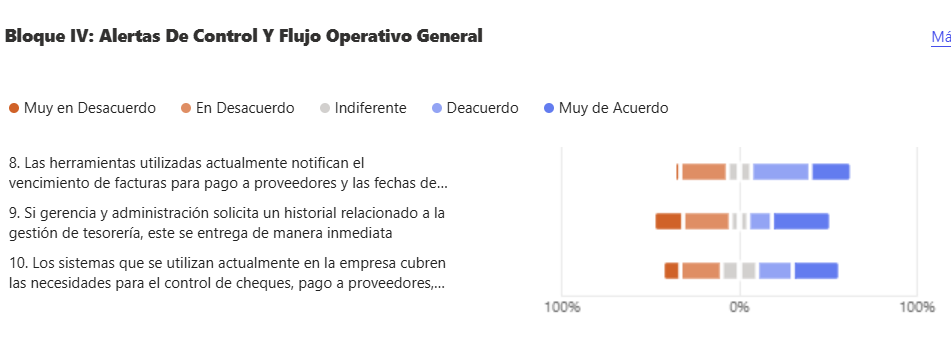
\includegraphics[width=\textwidth]{./imagenes/image22.png}
\end{figure}

\begin{table}[H]
\small
\begin{flushleft}
    \textbf{Tabla Anexo C4}\\[0.2cm]
    \emph{Bloque IV (Porcentajes Tres preguntas)}
\end{flushleft}
\renewcommand{\arraystretch}{1.0}
\centering
\begin{tabular}{
    >{\raggedright\arraybackslash}p{2.6cm} 
    >{\raggedright\arraybackslash}p{1.6cm} 
    >{\raggedright\arraybackslash}p{1.6cm} 
    >{\raggedright\arraybackslash}p{1.6cm} 
    >{\raggedright\arraybackslash}p{2.0cm} 
    >{\raggedright\arraybackslash}p{2.3cm} 
    >{\raggedright\arraybackslash}p{1.8cm}
}
\toprule
\textbf{Preguntas} & \textbf{Muy de\newline Acuerdo} & \textbf{De\newline Acuerdo} & \textbf{Indiferente} & \textbf{En\newline Desacuerdo} & \textbf{Muy en\newline Desacuerdo} & \textbf{Sin\newline Respuesta} \\
\midrule
P.8 & 7 & 10 & 4 & 8 & 1 & 0 \\
P.9 & 10 & 4 & 3 & 8 & 5 & 0 \\
P.10 & 8 & 6 & 6 & 7 & 3 & 0 \\
\midrule
\textbf{Suma Bloque} & \textbf{25} & \textbf{20} & \textbf{13} & \textbf{23} & \textbf{9} & \textbf{0} \\
\textbf{Total (\%)} & \textbf{27.8\%} & \textbf{22.2\%} & \textbf{14.4\%} & \textbf{25.6\%} & \textbf{10.0\%} & \textbf{0.0\%} \\
\bottomrule
\end{tabular}
\end{table}